\chapterfont{\color{DarkBlue}}  % sets colour of chapter
\sectionfont{\color{DarkBlue}}  % sets colour of sections
\subsectionfont{\color{DarkBlue}}  % sets colour of subsections

\renewcommand\pcolor{DarkBlue}
\renewcommand{\headrule}{\hbox to\headwidth{%
		\color{DarkBlue}\leaders\hrule height \headrulewidth\hfill}} % color of title
\fancyfoot[LE,RO]{\thepage}

{ \Large \leftwatermark{
		\put(-67,-66.5){ 1 }
		\put(-67,-91.5){ 2 }
		\put(-67,-116.5){ 3 }
		\put(-76.5,-151){
\includegraphics[scale=0.8]{img/thumbindex/thumbindex_DarkBlue.eps}}  
		\put(-67,-141.5){{\color{white} 4 }}
		\put(-67,-166.5){ 5 }
		\put(-67,-191.5){ 6 }
	} \rightwatermark{
		\put(350.5,-66.5){ 1 }
		\put(350.5,-91.5){ 2 }
		\put(350.5,-116.5){ 3 }
		\put(350.5,-151){
\includegraphics[scale=0.8]{img/thumbindex/thumbindex_DarkBlue.eps}}  
		\put(350.5,-141.5){ {\color{white} 4 } }
		\put(350.5,-166.5){ 5 }
		\put(350.5,-191.5){ 6 }
}}

\chapter[Deconvolution of bulk blood eQTL effects into immune cell sub-populations]{Deconvolution of bulk blood eQTL effects into immune cell sub-populations}

\chaptermark{}
\label{chap:chapter4-deconvolution}



\hfill \underline{BMC Bioinformatics} 2020 June 12; Volume 21: p1-23.

\hfill DOI: \href{https://doi.org/10.1186/s12859-020-03576-5}{s12859-020-03576-5}


\noindent
\\
\\
Raul Aguirre-Gamboa1\textsuperscript{1,\#}, Niek de Klein\textsuperscript{2,\#}, Jennifer di Tommaso\textsuperscript{1,\#}, Annique Claringbould\textsuperscript{2},Monique van der Wijst\textsuperscript{2}, Dylan de Vries\textsuperscript{2}, Harm Brugge\textsuperscript{2}, Roy Oelen\textsuperscript{2}, Urmo Võsa\textsuperscript{1,3}, Maria Zorro\textsuperscript{1}, Xiaojin Chu\textsuperscript{1,4}, Olivier B. Bakker\textsuperscript{1,2}, Zuzanna Borek\textsuperscript{1}, Isis Ricaño-Ponce\textsuperscript{1}, Patrick Deelen\textsuperscript{2,5}, Cheng-Jiang Xu\textsuperscript{4}, Morris Swertz\textsuperscript{1,5}, Iris Jonkers\textsuperscript{1}, Sebo Withoff\textsuperscript{1}, Irma Joosten\textsuperscript{6}, Serena Sanna\textsuperscript{1}, Vinod Kumar\textsuperscript{1,7}, Hans J.P.M. Koenen\textsuperscript{6}, Leo A.B. Joosten\textsuperscript{7}, Mihai G. Netea\textsuperscript{7,8}, Cisca Wijmenga\textsuperscript{1}, BIOS Consortium, Lude Franke\textsuperscript{2,*},Yang Li\textsuperscript{1,4,7,§,*}
\\
\\
\noindent
1 University of Groningen, University Medical Center Groningen, Department of Genetics, Groningen, the Netherlands\\
2 Department of Genetics, Oncode Institute, University of Groningen, University Medical Center Groningen, Groningen, The Netherlands\\
3 University of Tartu, Institute of Genomics, Tartu, Estonia\\
4 Centre for Individualised Infection Medicine (CiiM) \& TWINCORE, joint ventures between the Helmholtz-Centre for Infection Research (HZI) a nd the Hannover Medical School (MHH), Feodor-Lynen-Str. 7, 30625 Hannover, Germany\\
5 University of Groningen and University Medical Center Groningen, Genomics Coordination Center, Groningen, The Netherlands\\
6 Department of Laboratory Medicine, Laboratory for Medical Immunology, Radboud University Medical Centre, Nijmegen, the Netherlands\\
7 Department of Internal Medicine and Radboud Center for Infectious Diseases, Radboud University Medical Center, Nijmegen, the Netherlands\\
8 Department of Genomics \& Immunoregulation, Life and Medical Sciences Institute (LIMES), University of Bonn, Bonn, Germany\\
\# These authors contributed equally to this work.\\
* These authors jointly directed this work.\\
§ Corresponding author: yang.Li@ helmholtz-hzi.de
\\
\\
\noindent
published: 2020 June 12.



\section*{Abstract}

Expression quantitative trait loci (eQTL) studies are used to interpret the function of disease-associated genetic risk factors. To date, most eQTL analyses have been conducted in bulk tissues, such as whole blood and tissue biopsies, which are likely to mask the cell type context of the eQTL regulatory effects. Although this context can be investigated by generating transcriptional profiles from purified cell sub-populations, the current methods are labor-intensive and expensive. Here we introduce a new method, \textit{Decon2}, a framework for estimating cell proportions using expression profiles from bulk blood samples (Decon-cell) followed by deconvolution of cell type eQTLs (Decon-eQTL). The estimated cell proportions from Decon-cell agree with experimental measurements across cohorts ($R \geq 0.77$). Using Decon-cell we can predict the proportions of 34 circulating cell types for 3,194 samples from a population-based cohort. Next we identified 16,362 whole blood eQTLs and deconvoluted cell type interaction (CTi) eQTLs using the predicted cell proportions from Decon-cell. CTi eQTLs show excellent allelic directional concordance with those of eQTL($\geq$ 96\%-100\%) and chromatin mark QTL ($\geq$ 87\%-92\%) studies that used either purified cell sub-populations or single-cell RNA-seq, outperforming the conventional interaction effect. Decon2 provides a method to detect cell type interaction effects from bulk blood eQTLs, which is useful in pinpointing the most relevant cell type for a certain complex disease. Decon2 is available as an R package and Java application (\url{https://github.com/molgenis/systemsgenetics/tree/master/Decon2}), and as a web tool (www.molgenis.org/deconvolution).


\section{Introduction}

For many of the genetic risk factors that have been associated to immune diseases by genome-wide association studies (GWAS), the molecular mechanism leading to disease remains unknown\cite{hindorffPotentialEtiologicFunctional2009}. Most of these genetic risk variants are located in the non-coding regions of the genome, implying that they play a role in gene regulation\cite{ionita-lazaSpectralApproachIntegrating2016,javierreLineageSpecificGenomeArchitecture2016}. Expression quantitative trait locus (eQTL) analysis provides a way to characterize the regulatory effect of these risk factors in humans, and many eQTL studies have now been carried out using bulk tissues, for example, whole blood\cite{westraSystematicIdentificationTrans2013,joehanesIntegratedGenomewideAnalysis2017}. However, bulk tissues comprise many different cell types, and gene regulation is known to vary across cell types\cite{rajPolarizationEffectsAutoimmune2014,petersInsightGenotypePhenotypeAssociations2016,naranbhaiGenomicModulatorsGene2015}. In recent years, efforts to describe eQTL effects in purified cell sub-populations have been carried out in specific cell types\cite{chenGeneticDriversEpigenetic2016}. Unfortunately, the length and cost of the study protocols have limited these studies to small sample sizes and only a few cell types. Current developments on single cell (sc) RNASeq technologies have given rise to sc-eQTLs, such approach although promising is still bound to a limited number of individuals limiting the number of detectable cell type (CT) eQTLs. Nevertheless, being able to pinpoint the particular CT in which a risk factor exerts an eQTL effect could help us to understand its role in disease.

Statistical approaches to detect CT effects using tissue expression profiles have mainly been developed to evaluate gene by environment interaction (GxE) terms, for example, being able to detect CT eQTLs for myeloid and lymphoid lineages using only whole blood gene expression and by evaluating the interaction between genotype and cell proportions for neutrophils and lymphocytes in whole blood\cite{westraCellSpecificEQTL2015}. A second study linked eQTL genes to proxy genes through correlation; these proxy genes were then associated with intrinsic or extrinsic factors, such as cell proportions or inflammation markers\cite{zhernakovaIdentificationContextdependentExpression2017}. However, these efforts focused on exploiting only one GxE term, or on indirectly linking the CT proportions to given eQTL instead of directly ascertaining the interaction between all the main cell proportions comprising the bulk tissue and genotype. Unfortunately, quantifying cell proportions, in particular for rare sub-populations (total abundance of $\leq 3\%$ in circulating white blood cells), is expensive and time-consuming. Hence, quantifying immune cell proportions in large functional genomics cohorts is not common practice.

Here we present and validate \textbf{Decon2}, a computational and statistical framework that can: (1) predict the proportions of known circulating immune cell sub-populations (\textbf{Decon-cell}), and (2) use these predicted proportions along with whole blood gene expression and genotype information to assign bulk eQTL effects into CT eQTLs (\textbf{Decon-eQTL}). Our two-step framework provides an improvement over previously published methods. Unlike earlier methods\cite{aranXCellDigitallyPortraying2017}, Decon-cell does not rely on any prior information of transcriptome profiles from purified cell sub-populations, as it only requires the quantification of the cell proportions comprising the bulk tissue, in this case whole blood. Decon-cell identifies  signature genes that correlate with cell proportions in a bulk tissue. Secondly, Decon-eQTL is the first approach in which all major cell proportions (the major cell types for which the sum of proportions per sample to approximately 100\%) of bulk blood tissue are incorporated into an eQTL model simultaneously. Decon-eQTL can then be used to systematically test for any significant interaction between each CT and genotype, while at the same time controlling the effect on expression of the other cell types.

We generated the Decon-cell predictive models using data from the  500FG cohort\cite{neteaUnderstandingHumanImmune2016}, where quantification of immune cell types was carried out using FACS\cite{aguirre-gamboaDifferentialEffectsEnvironmental2016} and RNA-Seq based bulk whole blood transcriptome profiles were available for 89 samples\cite{bakkerIntegrationMultiomicsData2018}. By using a cross-validation approach we were able to accurately predict 34 out of 73 cell subtypes using solely whole blood gene expression. For validation, we applied Decon-cell to three independent cohorts (Lifelines Deep\cite{tigchelaarCohortProfileLifeLines2015}, n = 627, Leiden Longevity cohort\cite{deelenGenomewideAssociationMetaanalysis2014}, n = 660 and the Rotterdam Study\cite{hofmanRotterdamStudy20162015}, n = 773) with both blood RNA-seq and measured cell proportion data available (neutrophils, lymphocytes and CD14+ monocytes and granulocytes). Additionally, we benchmarked Decon-cell prediction performance against two other existing methods that quantify immune cell composition using gene expression profiles from whole blood on these three independent cohorts. After showing that we can accurately predict circulating immune cell proportions, we applied Decon-cell to estimate cell proportions in 3,194 individuals from the BIOS cohort\cite{tigchelaarCohortProfileLifeLines2015,greevenbroekCrosssectionalAssociationInsulin2011,schoenmakerEvidenceGeneticEnrichment2006,willemsenNetherlandsTwinRegister2010}, in which both whole blood RNA-seq and genotypes were available. The BIOS cohort is a valuable resource for functional genomics studies where extensive characterization of the genetic component on gene expression\cite{zhernakovaIdentificationContextdependentExpression2017} and epigenetics\cite{bonderDiseaseVariantsAlter2017} have been performed. We integrated whole blood expression, genotype information and predicted cell proportion with Decon-eQTL, to deconvolute 16,362 significant whole blood cis-eQTLs top effects into CT interacting eQTLs (CTi eQTLs). These deconvoluted CTi eQTL results were comprehensively validated using transcriptome profiles from purified cell sub-populations\cite{adamsBLUEPRINTDecodeEpigenetic2012}, eQTLs and chromatin mark QTLs from purified cell types\cite{chenGeneticDriversEpigenetic2016}, and eQTLs from single-cell experiments\cite{wijstSinglecellRNASequencing2018}. We also systematically compared the performance of Decon-eQTL against previously published methods\cite{westraCellSpecificEQTL2015,zhernakovaIdentificationContextdependentExpression2017} that detect cell type eQTL effects using whole blood expression profiles. 

\begin{figure}[H]
	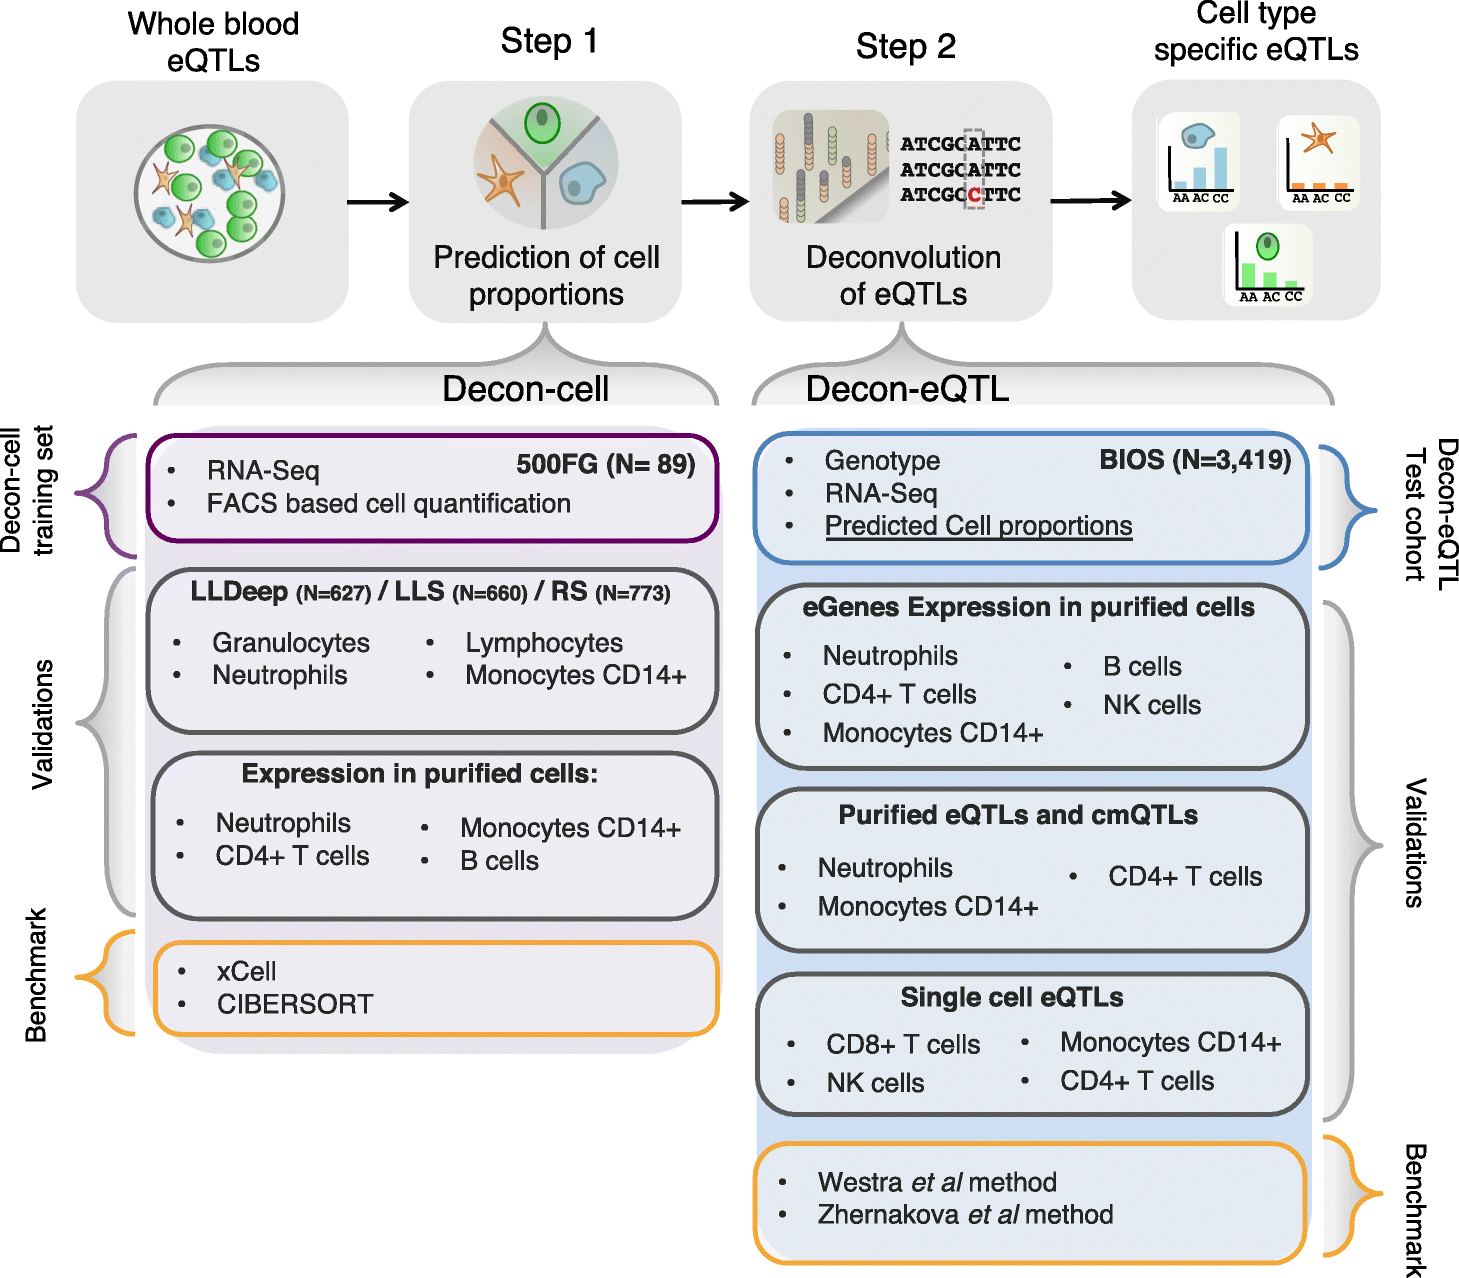
\includegraphics[width=\textwidth]{chapters/chapter4-deconvolution/img/fig1.png}
	\caption{\textbf{Workflow of application of Decon2 to predict cell counts followed by deconvolution of whole blood eQTLs.} Using whole blood expression and FACS data of 500FG samples, Decon-cell predicts cell proportions with selected marker genes of circulating immune cell subpopulations. Validations of Decon-cell were carried out on three independent cohorts for which measurements of neutrophils/granulocytes, lymphocytes and monocytes CD14+ were available along with expression profiles of whole blood. Benchmarking of Decon-cell was performed against CIBERSORT\cite{newmanRobustEnumerationCell2015} and xCell\cite{aranXCellDigitallyPortraying2017}. Decon-cell was applied to an independent cohort (BIOS) to predict cell counts using whole blood RNA-seq. Decon-eQTL subsequently integrates genotype and tissue expression data together with predicted cell proportions for samples in BIOS to detect cell type eQTLs. We validated Decon-eQTL using multiple independent sources, including expression profiles of purified cell subpopulations, eQTLs and chromatin mark QTLs (cmQTLs) from purified neutrophils, monocytes CD14+ and CD4+ T cells\cite{chenGeneticDriversEpigenetic2016}, and single-cell eQTL results\cite{wijstSinglecellRNASequencing2018}. Benchmarking of Decon-eQTL was carried out for comparison with a previously reported methods that detected cell type–eQTL effects using whole blood expression data, i.e. the Westra \textit{et al.}\cite{westraCellSpecificEQTL2015}}
	\label{decon_fig1}
\end{figure}

\section{Results}
\subsection{Decon-cell accurately predicts the proportions of known immune cell types}
In order to assign the cell types from which an overall eQTL effect from a bulk tissue sample (e.g. whole blood) comes from, we need three types of information: genotype data, tissue expression data, and cell type proportions (\textbf{Figure \ref{decon_fig1}}). Here, we propose a computational method for predicting the cell proportions of known immune cell types using gene signatures in whole blood expression data by employing a machine-learning approach. Decon-cell employs the regularized regression method elastic net25 to define sets of signature genes for each cell type. In other words, these signatures were selected as having the best prediction power for individual cell proportions. 

There are 89 samples in the 500FG cohort with both whole blood RNA-seq and quantification of 73 immune cell sub-populations by FACS available. This data was used to build the prediction models for estimating cell sub-populations by Decon-cell. First we determined which of the 73 cell sub-populations could be reliably predicted by Decon-cell. A within-cohort cross-validation strategy was employed by randomly dividing 89 samples (\textbf{Figure \ref{decon_fig1}}) into training and test sets (70\% and 30\% of the samples, respectively). After generating a model using each training set, we applied the prediction models of each cell type to the samples in the test sets. We compared the predicted and measured cell proportion for each cell type using Spearman correlation coefficients to evaluate the  prediction performance. We repeated this process 100 times and then used the mean of the correlation coefficient in all 100 iterations to evaluate the prediction performance. We were able to predict 34 out of 73 cell sub-populations using whole blood gene expression data at a threshold of mean $R \geq 0.5$ across all 100 iterations (\textbf{Figure \ref{decon_fig2}A}, \textbf{Supplementary Figure 1}, \textbf{Supplementary Table 1}). The number of signature genes selected in the models for predicting cell proportions varied across the cell types, ranging from 2 to 217 signature genes (\textbf{Supplementary Figure 2A}, \textbf{Supplementary Table 1}); and it was independent of the average abundance of these cell types in whole blood ($R = 0.02$, Spearman correlation coefficient, \textbf{Supplementary Figure2A}). In particular, cell types that are abundant in whole blood (granulocytes-neutrophils, CD4+ T-cells, CD14+ monocytes) were predicted with high confidence (correlation between predicted and measured values, $R \geq 0.73$). Remarkably, we were also able to predict a number of less abundant cell sub-populations, including NK cells, CD8+ T-cells, non-NK T-cells (CD3- CD56-), CD4+ central memory, CD4+ effector memory T-cells, and regulatory T-cells (\textbf{Supplementary Figure 2A}) as determined by FACS. Cell types with a low prediction performance ($R < 0.5$) are those that have few signature genes whose expression levels correlate sufficiently (i.e. absolute $R < 0.3$) with the actual cell proportions in whole blood (\textbf{Supplementary Figure 2B-C}). For each of the 34 predictable cell types, we used Decon-cell to build models for predicting their cell counts using all 89 samples from the 500FG cohort. These models were applied to 3,194 samples in an independent cohort (BIOS cohort), to predict cell proportions of circulating immune cell types for the subsequent deconvolution of eQTL effect. 

In addition to within-cohort validation, we tested our cell proportion models using three independent cohorts (LLDeep, $n = 627$, LLS, $n = 660$, $RS, n = 773$), for which cell type abundances were quantified using a Coulter counter for neutrophils (granulocytes for RS), lymphocytes, and CD14+ monocytes (\textbf{Figure \ref{decon_fig2}B}, \textbf{Supplementary Figure 3A-B}). In LLDeep we were able to accurately predict these three cell types with Spearman correlation coefficients of $R = 0.73$, $R = 0.89$, and $R = 0.73$, respectively.  For LLS and RS the prediction performance was also accurate for neutrophils and lymphocytes, but less so for monocytes ($R= 0.76$ for neutrophils, $R = 0.84$ for lymphocyte and $R = 0.50$ for CD14+ monocytes and proportions in LLS, $R = 0.74$ for granulocytes, $R = 0.83$ for lymphocytes and $R = 0.28$ for CD14+ monocytes and in RS). 

Next, in order to benchmark Decon-cell we have compared its prediction performance against two other existing tools that quantify the abundance of known immune cell types using bulk whole blood expression profiles: CIBERSORT\cite{newmanRobustEnumerationCell2015} and xCell\cite{aranXCellDigitallyPortraying2017}. We obtained the predicted proportions by CIBERSORT and enrichment scores of circulating immune cells by xCell for the samples in three different cohorts: LLDeep, LLS and RS (\textbf{Supplementary Figure 4A-B}). For each cell type, Decon-cell outperforms CIBERSORT and xCell (\textbf{Supplementary Figure 3B}). The scatterplots of predicted vs measured values  (\textbf{Supplementary Figure 3A}, and \textbf{Supplementary Figure 4 A-B}) further demonstrate that the better performance of Decon-cell is not due to cell proportion outliers.

Finally, we evaluated whether the signature genes showed CT expression in their relevant purified cell types, using the BLUEPRINT\cite{adamsBLUEPRINTDecodeEpigenetic2012} RNA-seq data from the purified cell sub-populations. We focused on cell types with more than three samples measured, which include neutrophils, CD14+ monocytes, CD4+ T-cells and B-cells. The signature genes showed overall higher expression in their relevant cell sub-populations compared to other cell sub-populations. Interestingly, the signature genes were also able to cluster the samples of the relevant CT using unsupervised hierarchical clustering (\textbf{Supplementary Figure 5A-D}). Together, our results demonstrated that the gene signatures identified by Decon-cell were predictive for the proportions of circulating immune cell sub-populations using only whole blood gene expression data.

To facilitate the cell proportion prediction of new samples using whole blood RNA-seq, we have made the Decon-cell prediction models and gene signatures available in an R package (Decon-cell) and as a web tool (www.molgenis.org/deconvolution). These two implementations allow the user to pre-process their RNA-seq expression counts and estimate cell proportions using the pre-established models for 34 cell types in whole blood. Morseso, Decon-cell R package allows the user to generate Decon-cell-like gene signatures to predict their own cell proportions, which requires the input of bulk expression profiles and cell proportions to generate new Decon-cell predictive models.

\begin{figure}[H]
	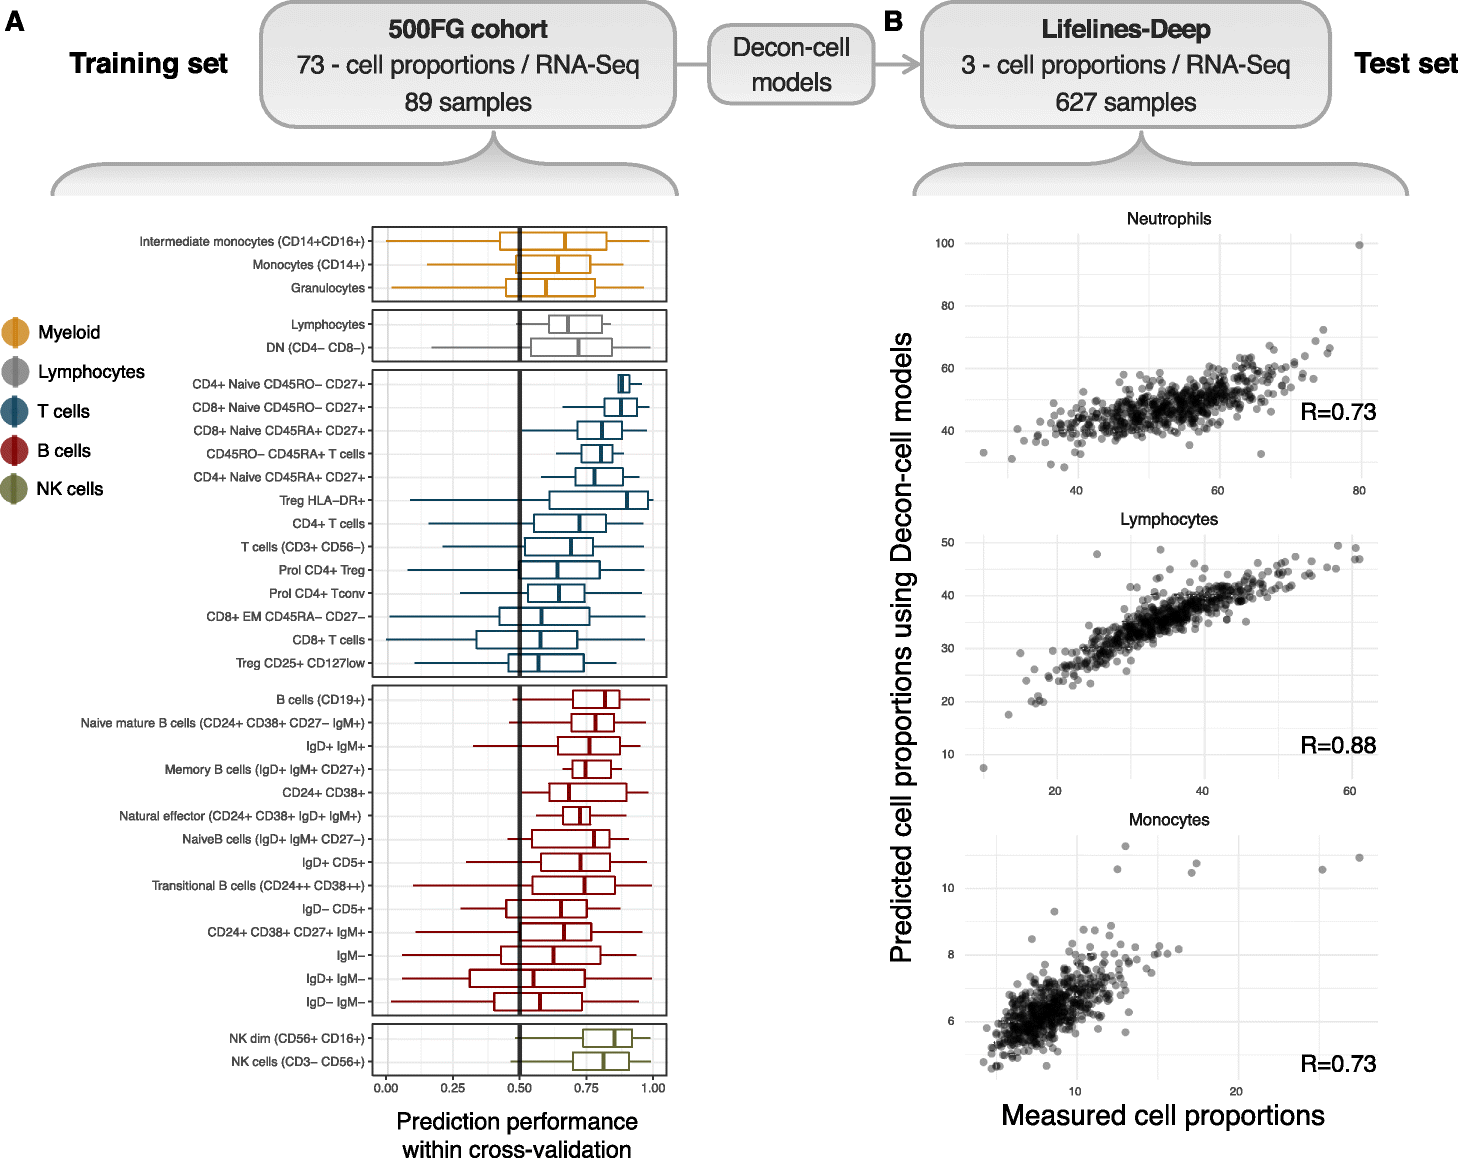
\includegraphics[width=\textwidth]{chapters/chapter4-deconvolution/img/fig2.png}
	\caption{\textbf{Prediction of cell proportions using whole blood transcriptome by Decon-cell.} (A) Distribution of prediction performance (Spearman correlation coefficient) of the 34 predictable cell types in 100 iterations of prediction within the 500FG cohort. (B) Cross-cohort validation in an independent Lifelines-Deep cohort (n = 627): the measured and predicted cell proportions for neutrophils (given by granulocytes in 500FG), lymphocytes and monocytes are compared}
	\label{decon_fig2}
\end{figure}


\subsection{Decon-eQTL identifies which cell types contribute to the whole blood eQTL effect}
As we know, eQTL analysis using whole blood bulk expression data fails to distinguish between a general eQTL that is present in all cell types and an effect that is mainly found in a subset of the cell types. We therefore propose a new approach to assign the overall bulk eQTL into CT effects, called Decon-eQTL (see Online Methods). By using the cell proportions in whole blood, it is possible to formally test if the genetic effect is interacting with the cell proportions. More explicitly, we include both the genotype and all major CT proportions of interest in a linear model and systematically test if there is a significant interaction effect between genotype and each of the cell proportions in the variation of gene expression in whole blood. At the same time the model used by Decon-eQTL controls the effect of the remaining cell types on gene expression. In this way, whole blood expression data, alongside genotypes and (predicted) cell proportions can be integrated to assign a CTi effect from a bulk eQTL(\textbf{Figure \ref{decon_fig1}}).

We applied Decon-eQTL to 3,198 samples (BIOS cohort) with transcriptome levels (RNA-seq), genotype information and cell proportions predicted by Decon-cell. Whole blood cis-eQTL mapping yielded 16,362 whole blood eQTLs (false discovery rate (FDR) $\leq 0.05$). For each of these whole blood cis-eQTLs, we applied Decon-eQTL with a focus on 6 major cell sub-populations: granulocytes, CD14+ monocytes, CD4+ T-cells, CD8+ T-cells, B-cells and NK cells. These cell types were selected as the sum of their relative percentages was close to 100\% and none of these cell type pairs had an absolute correlation coefficient $R \geq 0.75$. Decon-eQTL computationally assigned 4,139 CTi eQTLs from these sub-populations, reflecting 3,812 genes and 3,650 SNPs. 25\% of the whole blood eQTLs have a significant ($FDR \leq 0.05$) CTi eQTL effect given Decon-eQTL. The majority (31\%) of the total CTi eQTL effects detected were found to be associated to granulocyte proportions, possibly because granulocytes comprise ~70\% of circulating white blood cells (\textbf{Figure \ref{decon_fig3}A}). The majority (74\%) of CTi eQTLs detected by our method were assigned to a single cell type (\textbf{Supplementary Figure 6A}), similarly we find almost no sharing between cell types in single cell eQTLs from 112 individuals. However, it should be noted that these eQTL are likely not exclusively present for this particular cell type in biology, but that the statistical power given our sample size was sufficient to detect these interaction effects which we describe as CTi eQTL, in this particular cell type . Decon-eQTL was only able to find sharing of CTi eQTLs between cell types in a few cases, likely due to a lack of power of the interaction model. An example of such shared CTi eQTLs is on NOD2 gene, where Decon-eQTL was able to detect a strong granulocyte-eQTL effect alongside a smaller, opposite effect in CD14+ monocytes. This opposite effect has also been previously described in eQTL studies on purified CD14+ monocytes and neutrophils8. These results demonstrate that the effects of cell proportions on gene expression should be taken into account when interpreting eQTLs derived from bulk tissues.

\begin{figure}[H]
	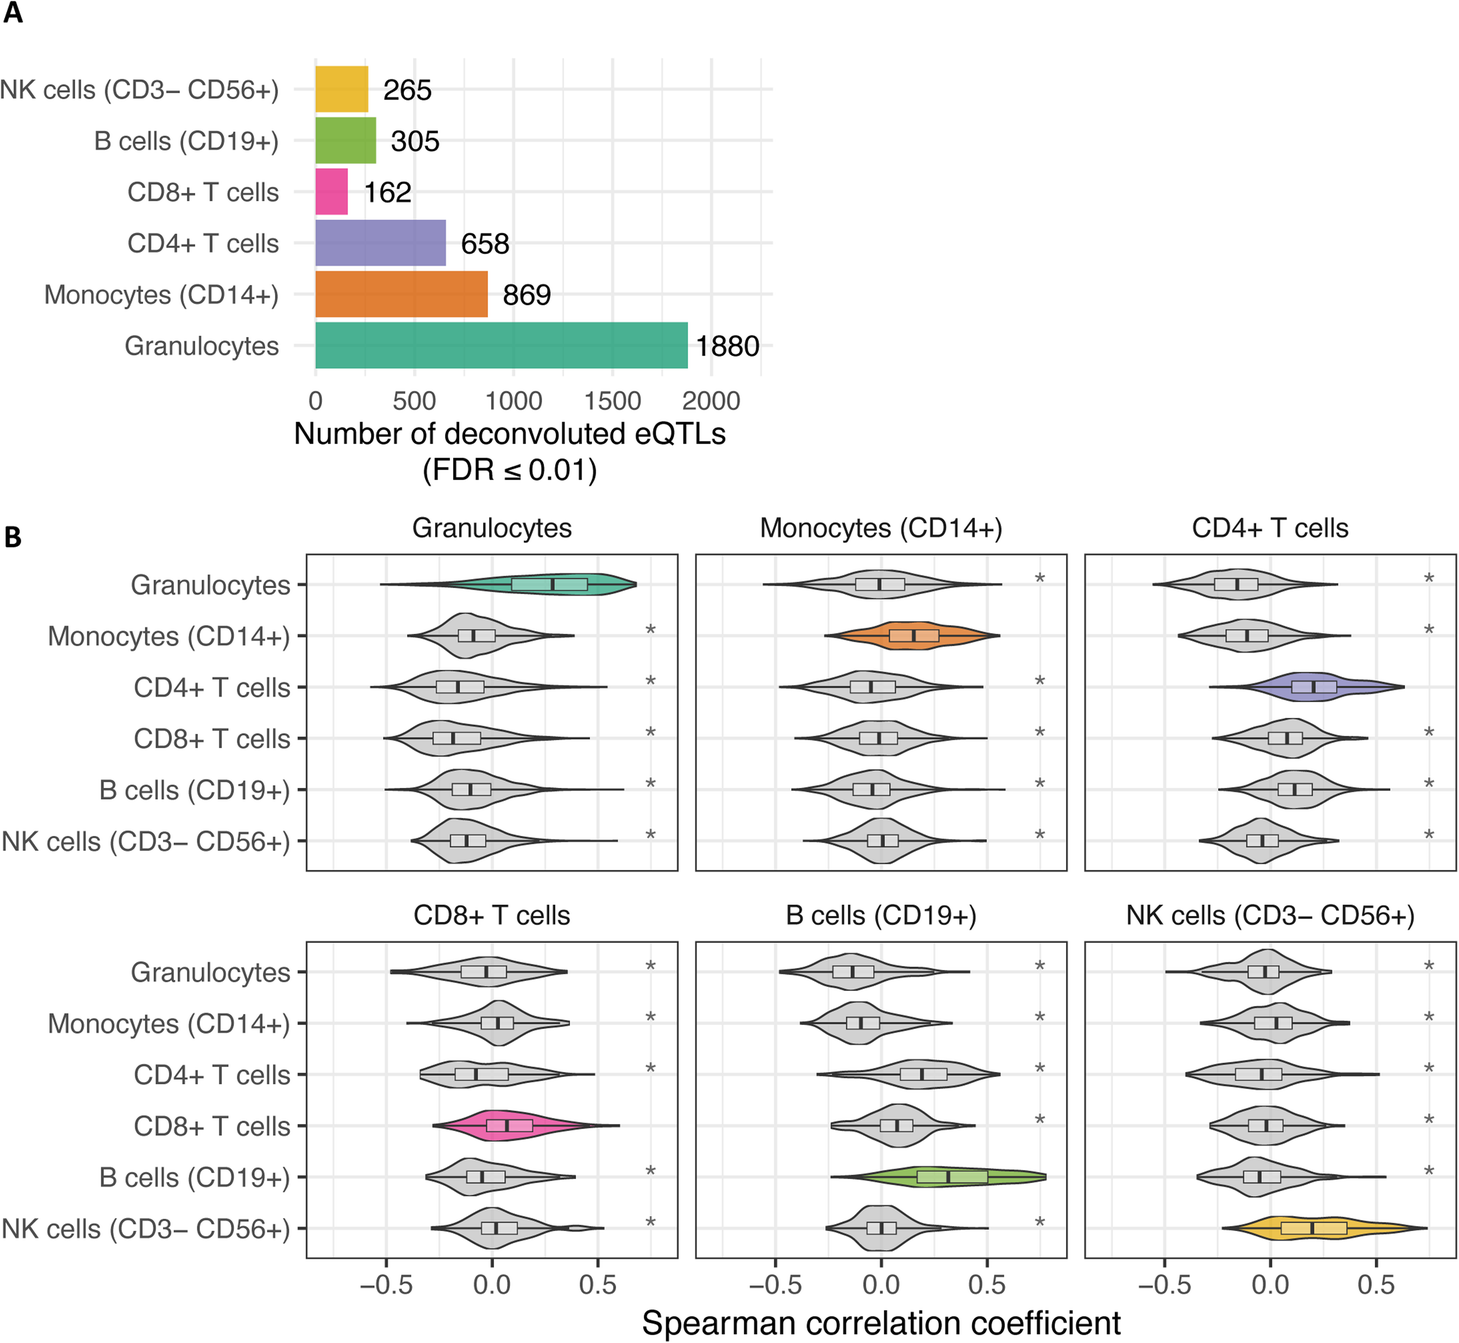
\includegraphics[width=\textwidth]{chapters/chapter4-deconvolution/img/fig3.png}
	\caption{\textbf{Deconvolution of whole blood eQTLs into CTi eQTLs}. Decon-eQTL detects CTi eQTLs by integrating proportions of cell subpopulations (predicted by Decon-cell), gene expression and genotype information. (A) Number of deconvoluted CTi eQTLs in each cell type using whole blood RNA-seq data of 3189 samples in BIOS cohort. (B) Distribution of Spearman correlation coefficients between expression levels of CTi eQTL genes and cell counts for each cell subpopulation. The CTi eQTL genes show positive and statistically higher correlation (Spearman) with the relevant cell type proportions as compared to the rest (T-test p-value $<$ 0.05) in an independent cohort (500FG)}
	\label{decon_fig3}
\end{figure}


\subsection{Decon-eQTL prioritizes genes to relevant cell types}
CTi eQTL genes are expected to have higher expression levels in their relevant cell types and therefore, their expression in whole blood should be correlated with the proportions of its given cell type. To test this, we evaluated if the expression levels of the CTi eQTL genes detected in the BIOS cohort were correlated with their relevant cell proportions and compared this to the correlation with non-relevant cell types. We calculated the Spearman correlation coefficients between the expression of the identified CTi eQTL genes and the measured cell proportions using the 500FG cohort ($n = 89$). Next, we compared the correlation coefficients obtained with those between expression and the remaining cell proportions. For each of the six evaluated cell sub-populations in Decon-eQTL, CTi eQTL genes had a significantly higher correlation with their relevant cell subpopulation than the other cell types (T test, p-value $\leq 0.05$) (\textbf{Figure \ref{decon_fig3}B}). As such, this result shows a significant association CTi eQTL ytgenes and the proportions of their relevant CT in an independent cohort.

Next, we evaluated whether the significant CT eQTL genes were over-expressed in their relevant cell subpopulation compared to eQTL genes that were found to be non-significant CTi eQTLs for the same cell type. For this purpose, we made use of the purified neutrophil, CD14+ monocyte, CD4+ T-cell and B-cell RNA-seq data from the BLUEPRINT dataset. We only include these cell types as they were the only ones with more than 3 samples measured. For each of the four cell types, we observed that the expression of CT eQTL genes detected by Decon-eQTL was significantly higher (T-test, p-value $\leq 0.05$) compared to the expression of non-significant Decon-eQTL genes (\textbf{Figure \ref{decon_fig4}A}). We also observed that the deconvoluted eQTL genes from granulocytes showed a relatively wider range of variation than the CT-eQTL genes from the other three sub-populations. We hypothesized that this could be explained by the fact that granulocytes comprise ~70\% of the cell composition in whole blood, thus giving us the power to detect eQTL for lowly-expressed genes in granulocytes. This was partly supported by the observation that the variation of expression in whole blood for granulocyte CTi eQTL genes was significantly greater than those CTi eQTL genes deconvoluted to the other five cell sub-populations (F test, p-value $\leq 0.05$, \textbf{Supplementary Figure 7}). 

Furthermore, by using publicly available transcriptome profiles (GSE7884027) of purified NK cells and CD4+ T cells, we assessed if the differentially expressed genes across the two cell types were enriched for eGenes of deconvoluted CT eQTLs. We observed that the CD4+ differentially expressed genes (Adjusted p-value $\leq 0.05$) were significantly enriched for CD4+ T cell eQTLs (Fisher exact p = $1.8 \times 10^{-17}$), whereas NK cell differential genes (Adjusted p-value $\leq 0.05$) were significantly enriched for NK cell eQTLs (Fisher exact p = $2.3 \times 10^{-18})$ as shown in \textbf{Figure \ref{decon_fig4}B}.

In summary, we were able to show that the eQTL genes detected by Decon-eQTL are transcriptionally active in their relevant cell type as that is where they are more highly expressed.

\begin{figure}[H]
	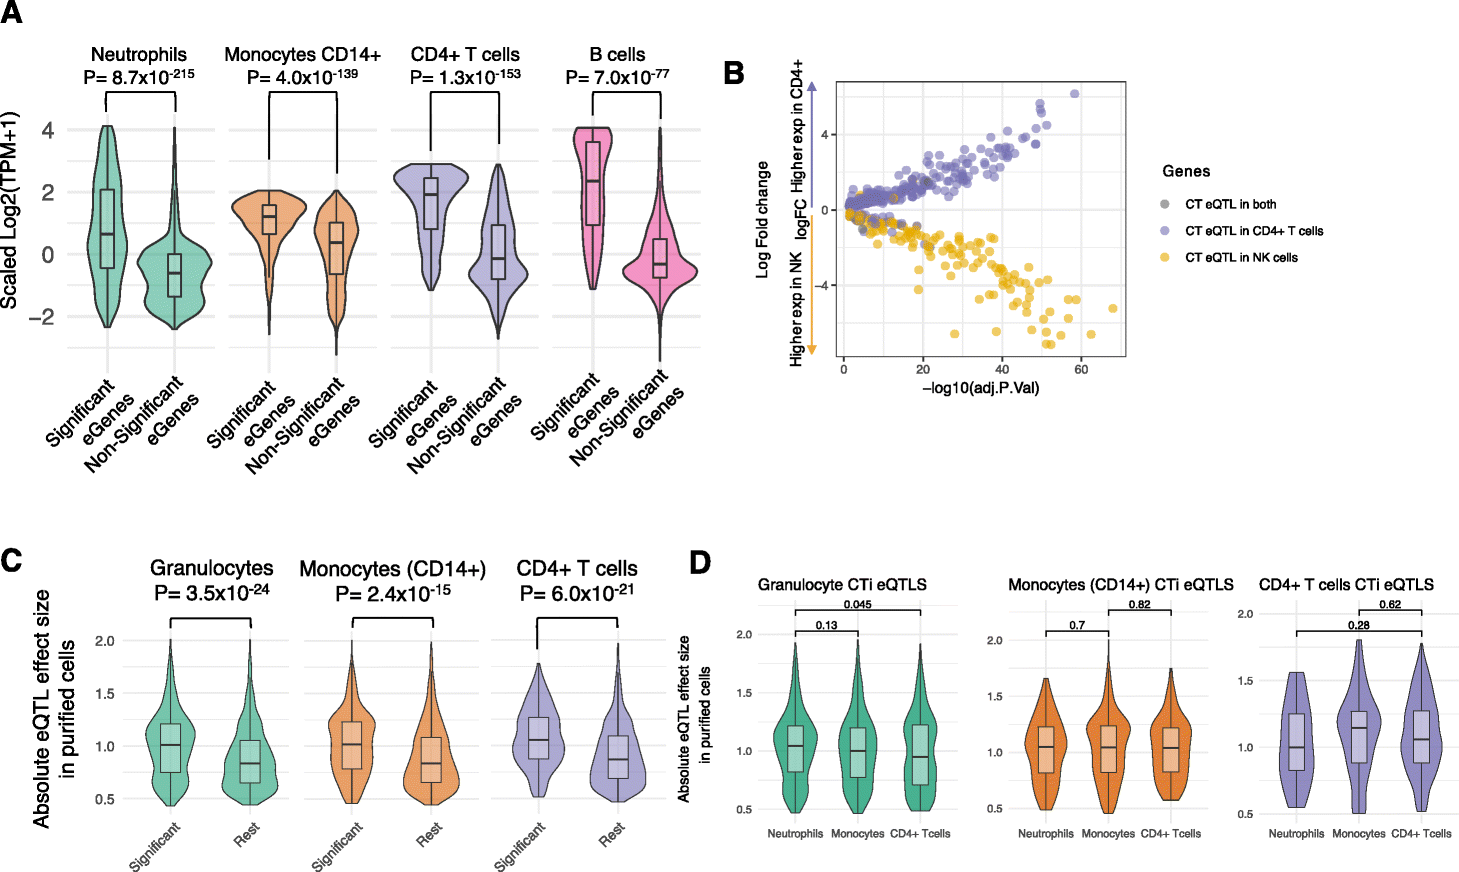
\includegraphics[width=\textwidth]{chapters/chapter4-deconvolution/img/fig4.png}
	\caption{\textbf{Validation of CTi eQTLs.} (A) The expression of CTi eQTL genes in purified cell subpopulations from BLUEPRINT\cite{adamsBLUEPRINTDecodeEpigenetic2012} are significantly higher in the relevant cell subpopulation when compared to other available cell subtypes (green for granulocyte eQTL genes showing expression for purified neutrophils; orange for monocytes; purple for CD4+ T cells; pink for B cells). (B) Genes differentially expressed (Adjusted p-value $\leq$ 0.5) between CD4+ T cells and NK cells are significantly enriched for CT eQTLs effects on CD4+ T cells (dots in purple, Fisher exact $-log_{10}(p) = 1.8 \times 10^{17}$) and NK cells (dots in yellow, Fisher exact $-log_{10}(p) = 2.3 \times 10^{18}$), respectively. (C) CTi-eQTLs (FDR $\leq$ 0.05) show significantly larger effect sizes in the purified cell eQTL data\cite{chenGeneticDriversEpigenetic2016} compared to the rest of the whole blood eQTLs for which we do not detect a cell type effect, as shown for deconvoluted granulocyte eQTLs in neutrophil-derived eQTLs (green),monocytes (orange) and CD4+ T cells (purple)}
	\label{decon_fig4}
\end{figure}


\subsection{CT eQTLs identified by Decon-eQTL in whole blood are replicated in purified cell eQTL datasets}
In order to validate the CT eQTLs defined by decon-eQTL, we utilized the eQTLs identified from purified neutrophils, CD4+ T-cells and CD14+ monocytes\cite{chenGeneticDriversEpigenetic2016}. We first compared the absolute effect sizes of eQTLs from purified cells that are also significantly deconvoluted CTi eQTLs with the effect sizes of eQTLs from purified cells that are also non-significant deconvoluted CTi eQTLs for this cell type. For all three cell populations, effect sizes in our deconvoluted CTi eQTLs were significantly higher compared to the effect size of eQTLs without a significant CTi eQTL (Wilcoxon test, p-value $\leq 0.05$, \textbf{Figure \ref{decon_fig4}C}). Next, we assessed the specificity of our deconvoluted CTi eQTLs by evaluating CTi eQTL effect sizes in non-relevant cell sub-populations. For example, we compared the effect sizes of deconvoluted granulocyte CTi eQTLs against those with non-significant deconvoluted granulocyte CTi eQTLs using the effect sizes of purified CD4+ T-cell eQTLs. Notably, we observed no statistically significant differences using effect sizes from non-relevant cell sub-populations (see off-diagonal comparisons in \textbf{Supplementary Figure 8}), further supporting the biological relevance of our deconvoluted CTi eQTLs. However, when comparing the effect sizes in purified eQTLs of only significant CTi eQTLs across all three available cell sub-populations, we were not able to find significant differences (\textbf{Figure \ref{decon_fig4}D}). For example, the effect size of neutrophils CTi eQTLs is the same across neutrophils, monocytes CD14+ and CD4+ T cells.

To further demonstrate that the CTi eQTLs assigned by Decon-eQTL are biologically meaningful, we have made use of the K27AC and K4ME1 epigenetic QTLs characterized in purified neutrophils, CD4+ T-cells and monocytes CD14+\cite{chenGeneticDriversEpigenetic2016}. In a similar fashion as the above comparison of effect sizes with purified eQTLs, we compared the absolute effect sizes from both K27AC and K4ME1 QTLs from eQTLs for which Decon-eQTL detects a significant CTi effect against the rest of whole blood eQTLs. We observed that for corresponding cell types, e.g. evaluating granulocyte CT eQTLs in K27AC QTLs from purified Neutrophils, the distribution of the absolute effect sizes is significantly higher for the chromatin mark QTLs (cmQTLs) than those non-significant CT eQTLs, which provide an epigenetic evidence that  our method is able to assign correctly the cell type eQTL effects, as shown in the diagonal comparisons in both K27AC QTLS (\textbf{Supplementary Figure 9}) and for K4ME1 QTLs (\textbf{Supplementary Figure10}). Notably, we observed that for the non-relevant cell sub-populations only one comparison, i.e. granulocytes v.s. CD14+ monocytes, show statistically significant higher effect sizes for K27AC QTLs and K4ME1 QTLs. For the rest of the non-relevant comparisons in the off-diagonal of both \textbf{Supplementary Figure 9} and \textbf{Supplementary Figure 10}, there are no statistically significant differences. Comparing the eQTL effect sizes in purified KC27AC and K4ME1 QTLs of only significant CTi eQTLs across all three available cell sub-populations shows that the effect sizes from the relevant cell type are  significantly stronger for all pairings except between granulocytes and CD14+ monocytes (\textbf{Supplementary Figure 11}).

In addition to the comparison of effect sizes, we compared the allelic concordance between deconvoluted eQTLs and eQTLs from purified cell subtypes9. For each available cell type (neutrophils, CD14+ monocytes, and CD4+ T cells), we evaluated whether the direction of the eQTL effect on deconvoluted CT eQTLs was the same as the one observed from purified cell sub-populations. The allelic concordance between the deconvoluted eQTLs and purified eQTLs was high across cell types: 99\% for granulocyte eQTLs (compared to neutrophil eQTLs), 96\% for CD14+ monocytes eQTLs, and 99\% for CD4+ T cells (\textbf{Figure \ref{decon_fig5}A}). These rates of allelic concordance are significantly higher for granulocyte and CD4+ T-cell CTi eQTLs compared to those between whole blood eQTLs and eQTLs from purified cell sub-populations (\textbf{Figure \ref{decon_fig5}B}, Neutrophils, Fisher exact p-value = $3.91 \times 10^{-106}$, CD4+ T cells Fisher exact p-value = $0.005$),  whereas the allelic concordance for deconvoluted CD14+ monocyte eQTLs is the same as for whole blood eQTLs and purified CD14+ monocyte eQTLs (\textbf{Figure \ref{decon_fig5}B}). We also compared the allelic concordance of deconvoluted CTi eQTLs of a certain cell type against the eQTLs of non-relevant purified sub-populations. Interestingly, the allelic concordance across non-relevant cell subtypes is consistently lower (off-diagonal \textbf{Supplementary Figure 12}, bonferroni corrected fisher exact p-value $< 0.0001$ for all comparisons). The higher allelic concordance across cell types was seen between deconvoluted granulocyte eQTLs and CD14+ monocyte eQTLs with a 95\% allelic concordance, which shows that the direction of effect is often shared between related cell types.

\begin{figure}[H]
	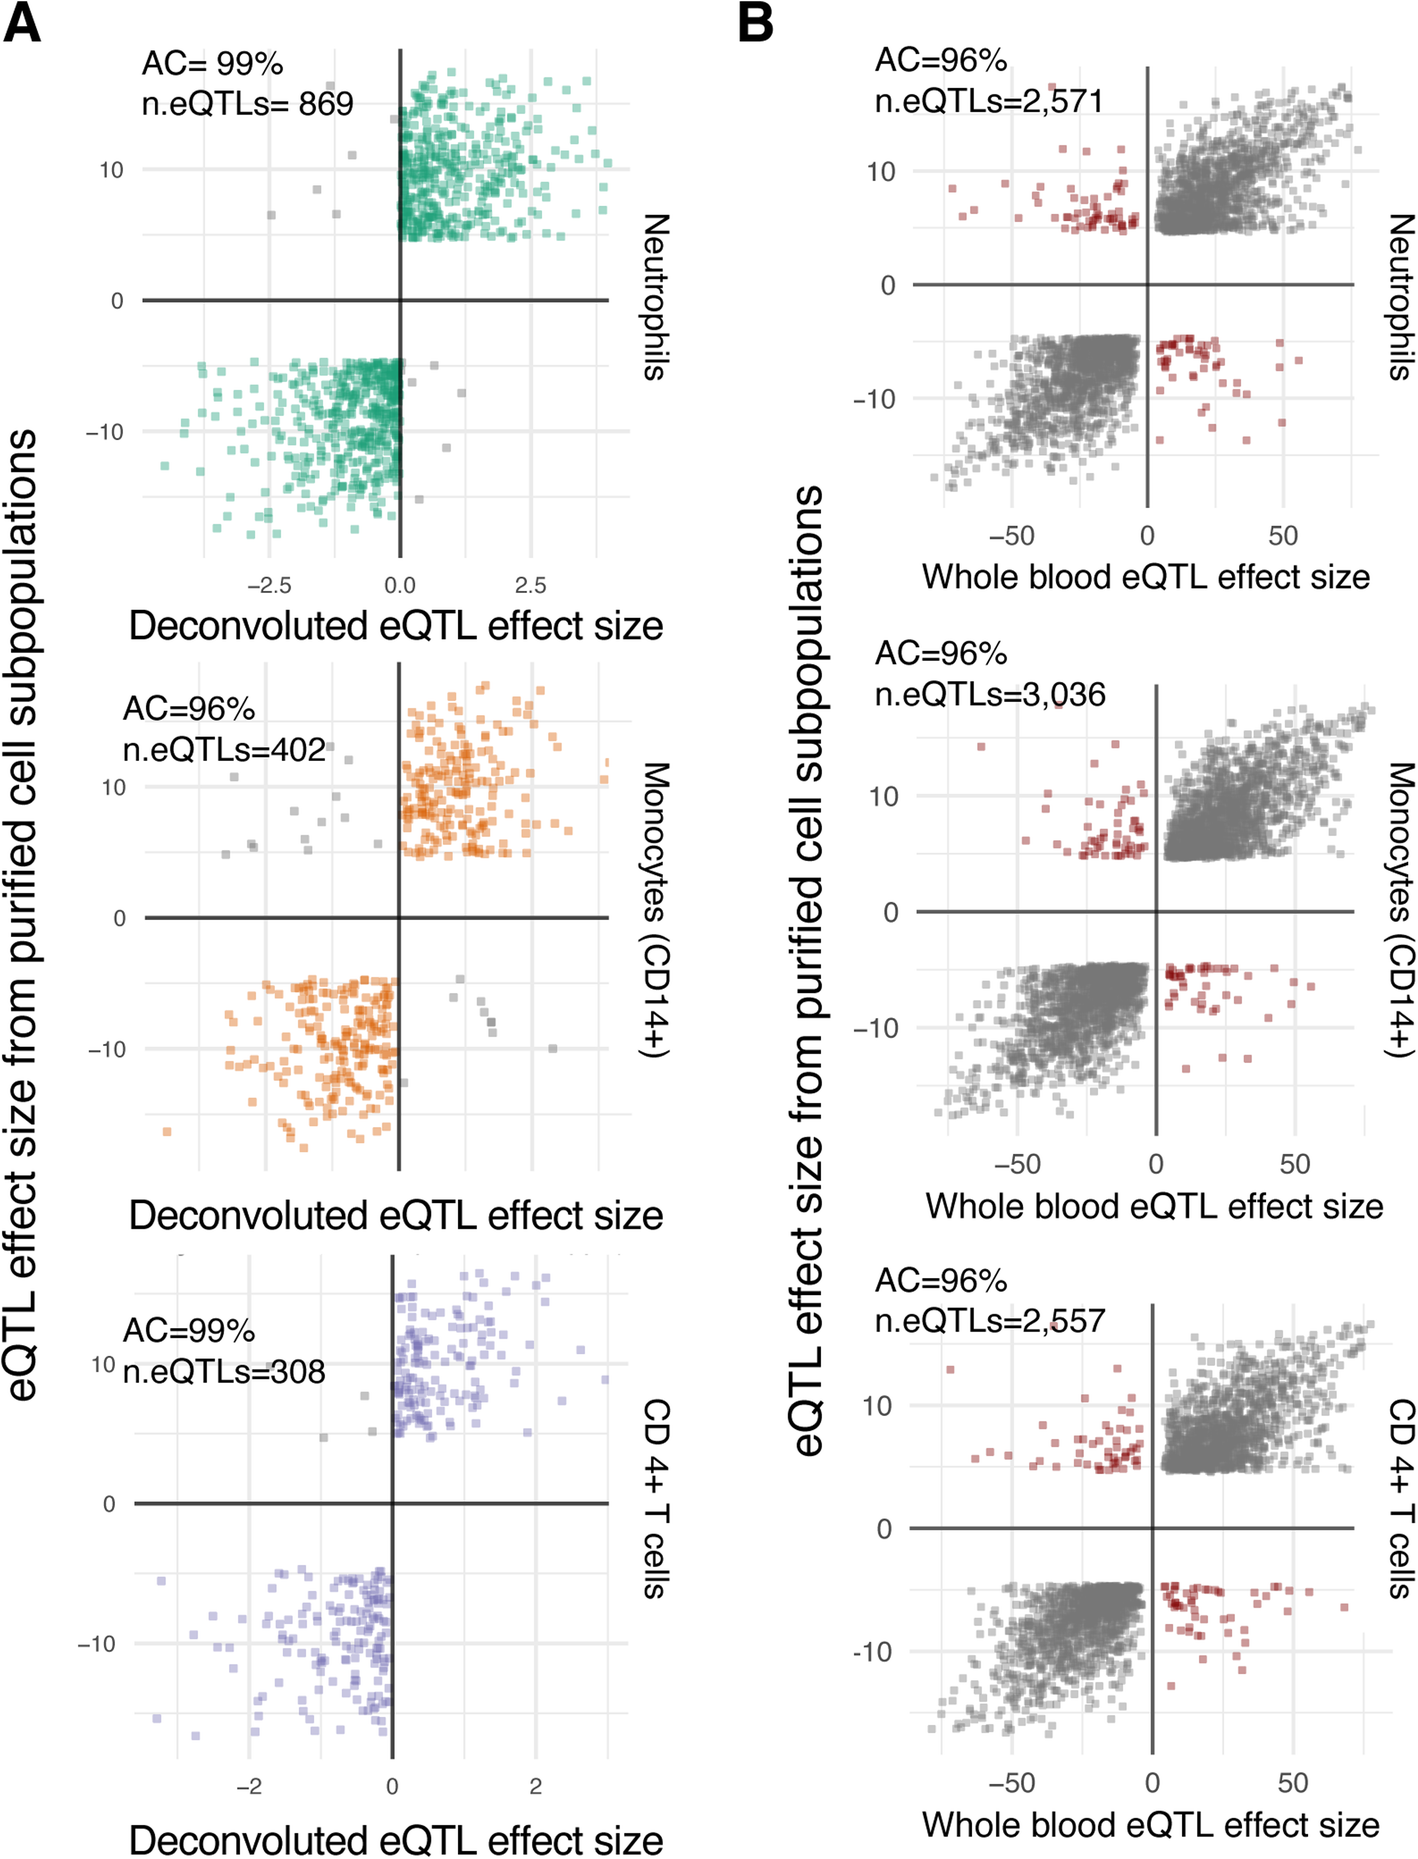
\includegraphics[width=\textwidth]{chapters/chapter4-deconvolution/img/fig5.png}
	\caption{\textbf{Allelic concordance of CTi eQTLs with eQTLs from purified cells.} CTi eQTLs show high allelic concordance compared to eQTLs from purified cell subpopulations9. (A) for granulocyte eQTLs (green), CTi eQTLs achieved an allelic concordance of 99\% compared to eQTLs from purified neutrophils. Similarly, the allelic concordances were 96 and 99\% for CD14+ monocytes and CD4+ T cells, respectively. Except for monocytes, these values are higher than those observed for whole blood eQTLs when comparing to eQTLs from purified subpopulations, as shown in panel (B)}
	\label{decon_fig5}
\end{figure}

Finally, we evaluated the allelic concordance rates for CTi eQTLs assigned by Decon-eQTL and K27AC QTLs from purified cell sub-populations, where we observed a consistently high allelic concordance rate: 92\% for granulocyte eQTLs (in purified Neutrophils), 87\% for CD14+ monocytes and 92\% for CD4+ T cells (boxed diagonal comparisons in \textbf{Supplementary Figure 13}). These concordance rates are significantly higher than the ones between the whole blood eQTLs and K27AC QTLs from purified cell sub-populations (\textbf{Supplementary Figure 14}) for neutrophils (Fisher exact test p-value $= 9.06 \times 10^{-14}$), CD14+ monocytes (Fisher exact test p-value $= 3.33 \times 10{-4}$), CD4+ T cells (Fisher exact test p-value $= 8.64 \times 10^{-9}$). Moreover we notice a consistent decrease in allelic concordance rates when assessing the concordance of CT eQTLs in K27AC QTLs of non-relevant cell sub-populations (off-diagonal compasons, \textbf{Supplementary Figure 13}). Together, the results from allelic concordance rates between deconvoluted CTi eQTLs and eQTLs/K27AC QTLs from purified cell sub-populations add a further layer of evidence supporting the biological relevance of deconvoluted CT eQTLs.

\subsection{CTi eQTLs identified by Decon-eQTL in whole blood show high allelic concordance with single-cell RNA-seq eQTLs}
To replicate the deconvoluted CT eQTLs in the cell subtypes that were not available in Chen \textit{et al.}\cite{chenGeneticDriversEpigenetic2016}. purified cell eQTLs, we utilized the recent single-cell RNA-seq eQTLs (sc-eQTLs) identified in CD14+ monocytes, NK cells, CD4+ T-cells, CD8+ T-cells, and B-cells\cite{wijstSinglecellRNASequencing2018} as well as new single cell data eQTL data that was processed in the same way. Combined, we used single cell eQTLs from 112 individuals. We selected all significant eQTLs for each of the cell types (Non Classical and Classical Monocytes were combined) and compared it to the direction of the eQTL effect given by Decon-eQTL. Overall we observed an allelic concordance of 96.42\% (\textbf{Figure \ref{decon_fig6}A}).

\subsection{Decon-QTL outperforms conventional interaction method}
To our knowledge, our approach is the first to model the effect of multiple components of bulk blood RNA-seq simultaneously in an attempt to fully deconvolute gene expression levels into more precise cell type x genotype effects. Previous studies used an interaction effect between genotype and cell proportions of one specific cell type to detect the cell type eQTL effects using whole blood gene expression\cite{westraCellSpecificEQTL2015}, or used the correlation of the eQTL effect with cell type proxy genes\cite{zhernakovaIdentificationContextdependentExpression2017}. 

The Westra et al method has often been used to detect cell type eQTL effects using bulk expression data and cell proportions\cite{davenportDiscoveringVivoCytokineeQTL2018,wilsonMappingTumorSpecificExpression2019,geeleherCancerExpressionQuantitative2018,glastonburyCellTypeHeterogeneityAdipose2019}. In brief, it focuses on the effect of the GxE interaction (where E represents cell proportions) for explaining the variation in gene expression, and it only incorporates one cell type at a time. To properly compare Decon-eQTL with the Westra \textit{et al.} method\cite{westraCellSpecificEQTL2015}, coined here ‘Westra method’, both methods were applied to the BIOS cohort, where we detected CT eQTLs for the six cell sub-populations. Replication of CT eQTLs from Westra method was done in the same way as described above for Decon-eQTL. We observed that the eGenes (i.e. genes with eQTLs) detected by the Westra method are significantly higher expressed for granulocytes ($p = 3.0 \times 10^{-12}$, observed in purified neutrophils), CD4+ T cells ($p = 5.0 \times 10^{-13}$) and B cells ($p = 5.1 \times 10^{-11}$), but not for CD14+ monocytes ($p = 1$, see \textbf{Supplementary Figure 15A}). Next, we found that the distribution of effect sizes in eQTLs from purified cells is significantly higher for the CT eQTLs detected using the Westra et al method when compared to the rest of the whole blood eQTLs ($p = 2.2 \times 10^{-47}$, $p = 9.6 \times 10^{-08}$, $p = 1 \times 10^{-47}$ for Neutrophils, Monocytes and CD4+ T cells respectively, boxed-diagonal comparisons in \textbf{Supplementary Figure 15B}) showing similar results as the ones from Decon-eQTL (\textbf{Supplementary Figure 8}).

When comparing the allelic concordance rates between the direction of effects given by the interaction term from the Westra method and those found in eQTLs from purified cell sub-populations, we observed that the allelic concordance for granulocytes eQTLs (99\%, evaluated in neutrophils, $p > 0.05$) and for CD4+ T cells 93\% (p $>$ 0.05), \textbf{Supplementary Figure 17}) is comparable to those observed for Decon-eQTL (\textbf{Figure \ref{decon_fig4}A}). Conversely, the allelic concordance rate for the CD14+ monocytes is only 62\%, significantly lower than the results from Decon-eQTL(96\%, $p = 0.001$). Finally, for granulocytes, CD4+ T cell eQTLs and monocytes, we have overlapped the the results from Westra method and Decon-eQTL with the eQTLs from purified cell types\cite{chenGeneticDriversEpigenetic2016} (\textbf{Supplementary Figure 17}). For all three cell types, we found that Decon-eQTL is able to detect a larger number of eQTLs. For Neutrophils the Westra method has a higher replication rate (fisher $p-value = 0.002$), for monocytes the methods had the same replication rate (fisher p-value $= 0.737$), and for CD4+ T-cells Decon-eQTL had a better replication rate (p-value $= 7.47 \times 10^{-12}$). 

Finally, we compare the difference in allelic concordance with single cell eQTLs. The overall allelic concordance of Decon-eQTL CTi QTLs with single cell eQTLs (96.42\%, Fig 6A) is higher than the one achieved by the Westra model ($p = 1.235 \times 10^{-08}$), where we observed an overall allelic concordance of 84.67\% (Fig 6B). For both non-classical Monocytes (fisher p-value $= 0.045$) and CD4+ T-cells (fisher p-value $= 7.896 \times 10^{-07}$) Decon-eQTL has a significantly better allelic concordance, for CD8+ T-cells (fisher p-value $= 0.230$), classical Monocytes (fisher p-value $= 0.0513$), B-cells (fisher p-value $= 0.055$) and NK cells (fisher p-value $= 0.242$) there is no significant difference, nevertheless for NK cells, classical Monocytes, and CD8+ T cells, Decon-eQTL show a higher allelic concordance (93.8\% vs 83.9\%, 96.2\% vs 89.2\%, and 100\% vs 93.5\% respectively), while for B-cells it has lower concordance (33\% vs 100\%, \textbf{Figure \ref{decon_fig6}B}).

Overall, these results demonstrate that Decon-eQTL is able to detect more CTi eQTLs that can be replicated in purified eQTL dataset that previously reported methods, especially in not so abundant cell types such as CD14+ monocytes. However, the detection of interaction effects between genotype and cell proportions to dissect bulk (in this case whole blood) expression data and detect CTi eQTLs, remains an area of great opportunity that could still be explored. Mainly to the constantly increasing  number of samples present in functional genomic cohorts and the greater number of purified and single cell eQTL dataset that can be used for validation. 

\begin{figure}[H]
	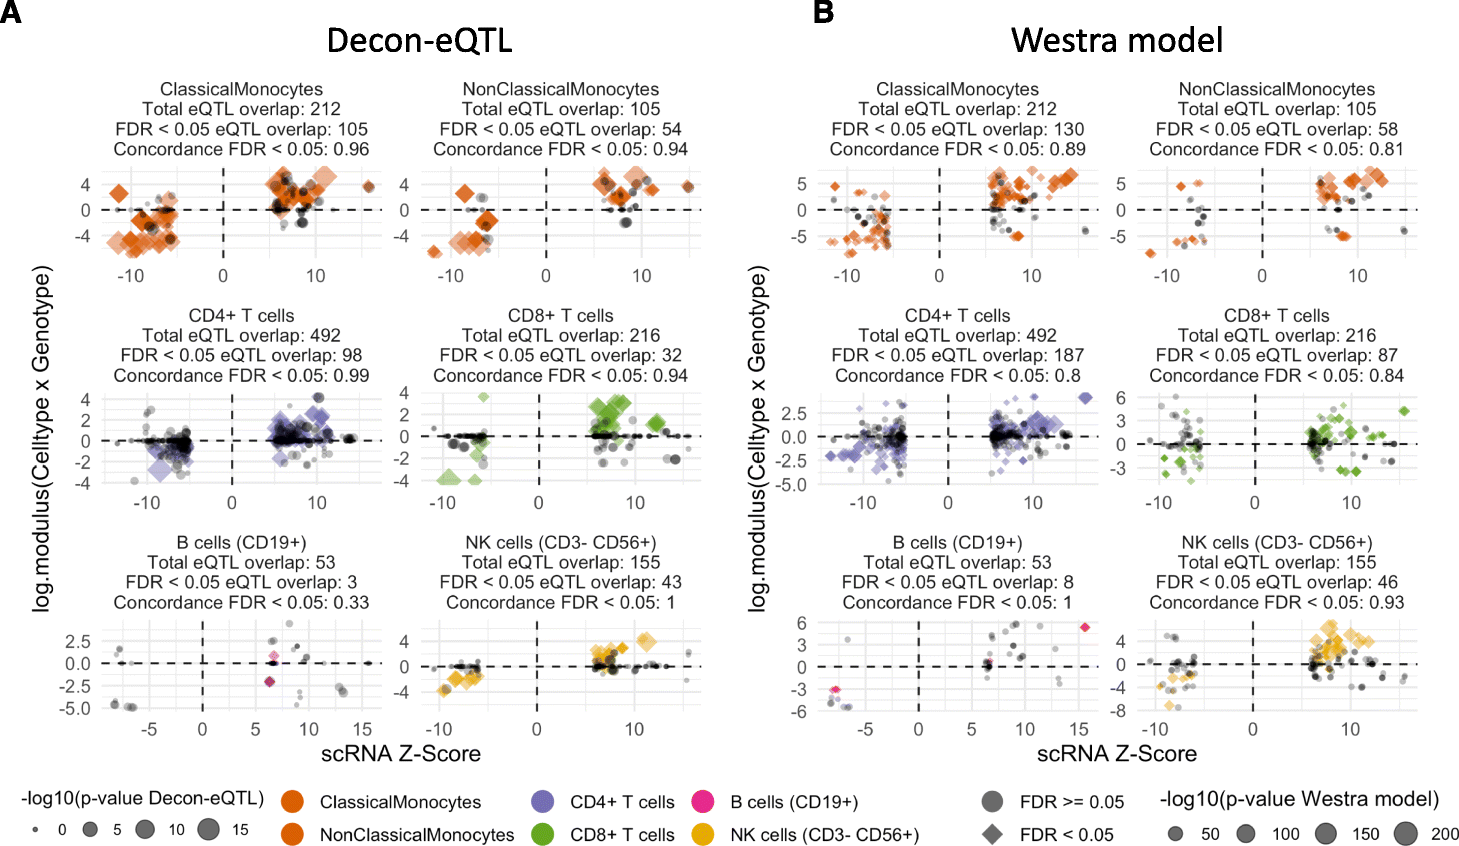
\includegraphics[width=\textwidth]{chapters/chapter4-deconvolution/img/fig6.png}
	\caption{\textbf{Allelic concordance of CTi eQTLs with eQTLs from single cell RNAseq.} (A) Comparison in allelic direction between CTi eQTLs and eQTLs from single cell RNAseq experiments in 6 cell types. (B) Comparison in allelic direction between Westra model eQTLs and single cell eQTLs. In both panels coloured diamonds are FDR $<$ 0.05, grey circles are FDR $geq$ 0.0 in the single cell data, and the size is the $-log_{10}(p-value)$ of the predicted cell type interacting eQTLs}
	\label{decon_fig6}
\end{figure}

\section{Discussion}
We have developed a novel statistical framework, Decon2, which predicts the proportions of known immune cell subtypes using gene expression levels from whole blood (Decon-cell). Subsequently, these predicted cell proportions, together with genotype information and expression data, can be used to deconvolute a whole blood  eQTL effect into cell type interacting effects (Decon-eQTL). Using a set of samples with both whole blood RNA-seq data and cell frequencies of 73 cell sub-populations, we demonstrated that Decon-cell was able to predict 34 independent cell sub-populations. The performance of Decon-cell has been validated using multiple independent cohorts and benchmarked with existing methods. The obtained Decon-cell models were applied to a cohort of 3,189 samples with whole blood RNA-seq available, resulting in predicted cell counts for these samples. By integrating bulk expression data, genotype and predicted cell counts of BIOS cohort,  Decon-eQTL was able to dissect whole blood eQTL effect into CTi eQTLs without purifying immune cell sub-populations. Again the results of Decon-eQTL were validated by using several independent data types: 1) eQTLs from purified cell sub-populations, 2) chromatin QTLs purified cells 3) gene expression from purified cell types and 4) eQTLs derived from single cell protocols. Compared with existing methods, Decon-eQTL consistently show superior performance. To sum up, the proposed framework is useful for (re)-analyse both, existing and new bulk blood tissue datasets to detect CTi eQTL effects, and can be applied and tested on other tissues once cell count proportions become available. This cataloging and further interpreting the role of CTi eQTLs will improve our understanding of the functional role of SNPs associated with complex diseases, at the level of specific cell subtypes.

The main advantage of our method for predicting cell proportions by Decon-cell  is that it does not rely on the gene expression measured in purified cell subtypes when defining signature gene sets. Moreover, our method does not require the definition of marker genes based on their differential expression compared to other cell sub-populations unlike previously reported methods\cite{aranXCellDigitallyPortraying2017}. The signature genes defined by Decon-cell are determined by a completely unsupervised approach using a regularized regression to select an optimal combination of genes to accurately predict a certain circulating cell proportion. Although the majority of these marker genes are differentially expressed across purified cell sub-populations, not all of them are. Nevertheless, these signature gene sets are still correlated to the cell proportions in whole blood. In summary, we have shown that Decon-cell is able to accurately predict the proportions of circulating immune cell sub-populations in three independent cohorts and that within these cohorts it out-performs previously reported methods.

Our Decon-eQTL method for detecting a CTi eQTL effect with bulk blood tissue expression data is, to our knowledge, the first attempt to simultaneously model whole blood gene expression profiles into its major components. In contrast to a previous method, where single cell type  ($G \times E$) effects were evaluated one at a time\cite{westraCellSpecificEQTL2015,glastonburyCellTypeHeterogeneityAdipose2019}, Decon-eQTL incorporates all the major cell proportions simultaneously to better dissect the overall genetic effect of gene expression signal into cell subpopulation effects. We have shown that CTi eQTL genes found with Decon-eQTL have higher expression and higher effect sizes in purified neutrophils, CD14+ monocytes and CD4+ T-cells than non-CTi genes, and we find significantly higher allelic concordance for 2 out of 4 tested cell types with single cell eQTLs than with a conventional interaction model (Fig 6A and 6B). Moreover, we have also shown the biological relevance of the deconvoluted CTi eQTLs by validating our results on cmQTLs where CTi eQTLs have significantly higher effect sizes and its allelic concordance rates are significantly higher than those of whole blood eQTLs.  Finally, we have also demonstrated that Decon-eQTL can replicate sc eQTLs derived from single-cell RNA-seq data, showing a higher allelic concordance with sc-eQTLs compared to using only whole blood eQTL effects.

There are limitations in our method: the CTi eQTLs detected by Decon-eQTL tend to be exclusive eQTL for the specific CT suggesting that the CT with the strongest eQTL effect was selected by Decon-eQTL. This is  likely due to the partial collinearity present between CT proportions included in the model (as shown by their correlation structure in \textbf{Supplementary Figure 18A-B}). Thus, the genetic effect of one cell type might be masked by another CT with correlated cell proportion. The highest correlation coefficient among cell types included in the model was 0.75 (between granulocytes and B cells). Therefore, a caveat to this is that by deconvoluting CTi eQTLs for partially correlated cell proportions could lead to false negative results for the cell types with relatively weaker eQTL effects. 
In our model we included the six major blood cell types. There are many more cell types available, for which our method is not able to detect a CTi eQTL estimate. Furthermore, we only tested Decon-eQTL using genome-wide whole blood cis-eQTLs main effects. Such eQTLs effects are very likely shared across multiple cell types, however due to statistical power and co-linearity we are only able to detect its interaction with only one cell type (\textbf{Supplementary Figure 6A}), which is also seen in single cell eQTLs with limited (112) samples (\textbf{Supplementary Figure 6B}). Nevertheless, this does not imply that the CTi eQTL are exclusive for or only present in such cell type, as we observe in \textbf{Figure \ref{decon_fig4}D}, where the effect sizes of the significant CTi eQTLs in purified sub-populations are not significantly different across all three purified cell sub-populations. Yet this difference in effect size of CTi eQTLs between relevant and non-relevant cell types can be seen in histone modification QTLs as shown in \textbf{Supplementary Figure 11}, likely due to the cell type specificity of epigenetic marks. Lastly, Decon2 has only been tested in whole blood where large numbers of samples are available, and therefore it is not known how it will perform in other tissues such as solid like bulk tissues.

The proposed framework of Decon2 is generic for predicting cell sub-populations in bulk tissues (Decon-cell) and re-distribute the overall eQTL effect into cell types (Decon-eQTL). Both methods have been implemented in freely available software. In both an R package and a user interface-based webtool, the models for predicting cell subpopulation in whole blood constructed and validated in this work are provided for people interested in estimating immune cell sub-populations in whole blood in healthy people with western european ethnicity, as our models were built using a Dutch cohort (500FG). 

In summary, Decon2 is a computational method that can accurately assign CT effects in whole blood functional genomic cohorts, which can be applied to any dataset for which genotypes and expression data is available and could potentially aid the understanding of the molecular effects of genetic risk factors associated with complex diseases at the cell subpopulation level. Our method makes it possible to create CT gene regulatory networks that could explain the different effects that each CT has on a complex disease in a cost-efficient way. Since Decon2 only requires  gene expression and genotype information to deconvolute bulk blood eQTLs into CTi eQTLs, it is possible to re-analyze the existing bulk blood RNA-seq data for which genotypes are also available; in this scenario we would use Decon-cell to predict cell proportions in whole blood and obtain CT information on many more eQTLs from an increase in sample size. The methods behind Decon2 can potentially be generalized to use transcriptional profiles derived from any other type of bulk tissue in addition to whole blood, such as biopsies from tumors or other solid tissues implicated in complex disease etiology. However, it has not been tested in other tissues. Our methods can hence aid in the detection of genetic effects on gene expression in rare cell sub-populations in bulk tissues. 

\section{Methods}
\subsection{RNA-seq data collection in 500FG cohort}
We selected a representative subset of 89 samples from the 500 participants of the 500FG cohort, which is part of the Human Functional Genomics Project (HFGP). Our subset was balanced for age and sex given the original distribution in the cohort. RNA was isolated from whole blood and subsequently globin transcripts were filtered by applying the Ambion GLOBINclear kit. The samples were then processed for sequencing using the library preparation kit Illumina TruSeq 2.0. Paired-end sequencing of $2 \times 50-bp$ reads was performed on the Illumina HiSeq 2000 platform. The quality of the raw reads was checked using FastQC (http://www.bioinformatics.babraham.ac.uk/projects/fastqc/). Read alignment was performed with STAR 2.3.032,33, using the human Ensembl GRCh37.75 as reference, whilst the aligned reads were sorted using SAMTools\cite{liSequenceAlignmentMap2009}. Lastly, gene level quantification of the reads was done using HTSeq35.

\subsection{RNA-seq preparation and data processing in the BIOS cohort}
RNA was isolated from whole blood and subsequently globin transcripts were filtered by applying the Ambion GLOBINclear kit. Library preparation was performed using the Illumina TruSeq v2 library preparation kit. Next, Illumina HiSeq 2000 was used for paired-end sequencing of $2 \times 50 bp$ reads while pooling 10 samples per lane and expecting $>$ 15 million read pairs per sample. By using CASAVA read sets were generated, retaining only reads that passed Illumina Chastity Filter for further processing.
Quality control of the reads was evaluated using FastQC (http://www.bioinformatics.babraham.ac.uk/projects/fastqc/). Adaptor sequences were trimmed out using cutadapt (v1.1) using default settings. Low quality ends of reads were removed using Sickle (v1.200) (https://github.com/najoshi/sickle). 
Reads were then aligned using STAR 2.3.0e\cite{dobinSTARUltrafastUniversal2013}. All SNPs present in the Genome of the Netherlands (GoNL) with MAF $\geq 0.01$ were masked from the reads to avoid reference mapping bias. Read pairs with at most eight mismatches and mapping to at most five positions, were used. Quantification of counts per genes was done using Ensembl v.71 annotation (which corresponds to GENCODE v.16).

\subsection{Genotype data of the BIOS cohort}
Genotype information was independently generated by each of the cohorts, further details on data collection and methods used for genotyping can be found in their papers (CODAM\cite{damParentalHistoryDiabetes2001}, LLDeep\cite{tigchelaarCohortProfileLifeLines2015}, LLS\cite{deelenGenomewideAssociationMetaanalysis2014}, RS\cite{hofmanRotterdamStudy20162015} and NTR\cite{willemsenNetherlandsTwinRegister2010})

Genotypes were harmonized to GoNL with Genotype Harmonizer\cite{deelenGenotypeHarmonizerAutomatic2014}  and imputed using IMPUTE2\cite{howieFlexibleAccurateGenotype2009} using GoNL as reference panel. SNPs with an imputation score below 0.5, Hardy-Weinberg equilibrium P value smaller than $1 \times 10^{-4}$, a call rate below 95\% or a MAF smaller than 0.05 were filtered out. For further analysis only eSNPs from whole blood cis-eQTL top effects were subsequently used in Decon-eQTL. 

\subsection{Quantification of cell proportions in 500FG cohort}
The inclusion criteria and further description of the participants of the 500FG cohort can be found at http://www.humanfunctionalgenomics.org. A total of 73 manually annotated immune cell sub-populations were quantified using 10-color flow cytometry. To minimize biological variability, cells were processed immediately after blood sampling and typically analyzed within 2–3 hr. Cell populations were gated manually as previously described\cite{aguirre-gamboaDifferentialEffectsEnvironmental2016}.

\subsection{cis-eQTLs in the BIOS cohort}
For cis-QTL mapping, we tested association between genes and SNPs located within 250 kb of a gene center. SNPs with MAF $\geq 0.01$, call rate = 1 and Hardy–Weinberg equilibrium p-value $\geq 0.0001$ were included. eQTLs were declared to be significant at FDR $< 0.05$. Pre-processing of RNA-seq and QTL mapping was performed using a custom eQTL pipeline which has been previously described\cite{zhernakovaIdentificationContextdependentExpression2017}.

\subsection{Prediction of cell proportions using gene expression levels from bulk tissue (Decon-cell)}
For cell count prediction expression data is TMM normalized, log2(expression+1) transformed, and z-transformed (scaled). We proposed that the abundance of molecular markers such as gene expression could be used as proxies to predict cell proportions. This can be represented as:

\begin{equation}
C_{kj} = \beta_{ki} \cdot Y_{ij} + \epsilon_{kj}
\end{equation}

where expression data is $Y_{ij}$ for genes $i = 1, 2,..., G$, samples $j = 1, 2, ..., N$, cell count data is $C_{kj}$ for sample $j$ in cell type $k (k = 1, 2, ..., K)$, $\beta_{ki}$ represents the coefficients of gene $i$ in determining cell counts of cell type $k$ of a complex tissue, and $\epsilon_{kj}$ is the error term.
In order to select only the most informative genes for predicting cell counts, we implemented a feature selection scheme by applying an elastic net (EN) regularized regression25. In the EN algorithm, the $\beta_{ki} \cdot Y$ are estimated by minimizing:

\begin{equation}
\Vert C_{k}-\beta_{k} Y\Vert^2\ subject\ to\ (1 - \alpha) \Vert \beta_{k} \Vert^2 + \alpha \Vert \beta_{k} \Vert_{1} \leq  s
\end{equation}

$s$ is a tuning parameter that limits the number of features that will be included in the final predictor model. We estimate the best s per cell type by applying a 10-fold cross-validation approach, where the most optimal penalty parameter ($\alpha$) was obtained.

\subsection{Normalization and correction of gene expression data for deconvolution of eQTL effects}
Total read counts from HTSeq were first normalized using the trimmed means of M (TMM) values32. TMM expression values were log2 transformed. For predicting cell proportions, we used scaled expression data in both the 500FG and BIOS cohorts.
For the deconvolution of eQTLs, the expression was log2 transformed and corrected using a linear model for the effect of cohort, age, sex, GC content, RNA degradation rates, library size, and number of detected genes per sample. The corrected expression data is then exponentiated in order to maintain the original linear relationship across read counts (gene expression) and cell proportions.

\subsection{Deconvolution of eQTL effects (Decon-eQTL)}
Decon-eQTL models  the expression level in the bulk tissue by considering the genetic contribution of multiple  cell types present in the system. For identifying the CT eQTL effect, the interaction term between a particular cell type and genotype was tested for statistically significance contribution to the explained variance on the expression levels of particular gene, while accounting for the remaining cell proportions. 

If we consider a generic eQTL linear model for whole blood it can be described as:

\begin{equation}
y = \alpha + \beta\cdot g+\epsilon
\end{equation}

where $y$ is the measured gene expression, $\alpha$ the modeled non-genetic dependent expression, $g$ the genotype coded as 0, 1 or 2, $\beta\cdot g$ the genotype-dependent expression, and $\epsilon$ the error, e.g. unknown environmental effects. Here all three terms are modeling the effect of the mixture of different cell types present in blood. 

In an RNA-seq based gene expression quantification of a bulk tissue, one could express gene expression levels ($y$) as the sum of counts ($\Psi$) per K cell types:

\begin{equation}
y = \sum_{k=1}^{K} \Psi_{k}
\end{equation}

For every cell type the expression level has can be written as a generic eQTL model (equation 3) weighted by the cell proportions. $\Psi_{k}$ is a combination of the genetic and non genetic contribution of the cell type to $y$. The non-genetic contribution per cell type is $\beta \cdot c$ where $c$ is the cell count proportions. The genetic contribution is $\beta_{k} \cdot g \times c_{k}$. For $k$ cell types the expression then is 

\begin{equation}
y = \sum_{k=1}^K \Psi_{k} = \sum_{k}\cdot ( \beta_{k}\cdot c_{k} ) + \sum_{k} \cdot (\gamma_{k} \cdot g \times c_{k}) + \epsilon
\end{equation}

Where $y$ is the measured expression levels, $k$ is the total number of cell types, $c_{k}$ is the cell count proportions of cell type $k$, $g$ is the genotype, and $\epsilon$ is the error term. Since we are assuming a linear relationship between total gene expression and the levels of expression generated by each of the cell types composing a bulk tissue, the cell proportions are scaled to sum to 100\%, such that the sum of the effect of the cell types equals the effect in whole blood. Here we assume that the true sum of the cell counts should be very close to 100\% of the total PBMCs count, which is why we include the 6 cell types that together form the top hierarchy given the gating strategy used to quantify the cell sub-populations\cite{aguirre-gamboaDifferentialEffectsEnvironmental2016}. The genotype main effect is not included in the model as the sum of the genotype effect per cell type should approximate the main effect.

Because the contribution of each of the cell types to expression level $y$ can not be negative, we constrain the terms of the model to be positive by using Non-Negative Least Squares\cite{zhouPreconditionedGAORMethods2009,lawsonSolvingLeastSquares1995} to fit the parameters to the measured expression levels. However, if the allele that has a negative effect on gene expression is coded as 2, the best fit would have a negative interaction term, which would be set to 0. To address this we want the allele that causes a positive effect on gene expression to always be coded as 2. However, the effect of an allele can be different per cell type, therefore the coding of the SNP should also be different per cell type. Therefore, we run the model multiple times, each time swapping the genotype encoding for one of the interaction terms. The encoding that gives the lowest R-squared is then chosen as the optimal genotype encoding. For the encoding we limit the amount of genotypes that have an opposite genotypic encoding to maximum of one interaction term, as we have observed that there no significant difference compared to using all possible configurations and this limits the amount of models that have to be run from $k^2$  to $(2*k)+2$.

To test if there is a CT interaction effect we run the linear model of equation 5. and, for each CT, run the same model with the cell proportion x genotype interaction term removed. E.g. when testing two cell types the full model is

\begin{equation}
y = \beta_{1} \cdot c_{1}+\beta_{2} \cdot c_{2} + \gamma_{1} \cdot g \times c_{1} + \gamma_{2} \cdot g \times c_{2} + \epsilon
\end{equation}

and the two models with the interaction terms removed are 

\begin{equation}
\begin{aligned}
y = \beta_{1} \cdot c_{1} + \beta_{2} \cdot c_{2} + \gamma_{1} \cdot g \times c_{1}\ \ \ \ \ \ \ \ \ \ \ \ \ \ \ \ \  + \epsilon \\
y = \beta_{1} \cdot c_{1} + \beta_{2} \cdot c_{2}\ \ \ \ \ \ \ \ \ \ \ \ \ \ \ \ \ +\gamma_{2} \cdot g \times c_{1} + \epsilon
\end{aligned}
\end{equation}

For both the full model and the CT models we calculated the sum of squares using the different genotype configurations detailed above. For both the full and the CT models we then selected the genotype configuration with lowest sum of squares. Then, for each CT, we test if full model can significantly explain more variance than the CT model using an ANOVA.

We have then applied our strategy to 16,362 significant whole blood cis-eQTLs top effects that were detected using the BIOS cohort. We then correct the p-values for multiple testing using FDR by each of the cell types, e.i. Granulocyte eQTL p-values were corrected for 16,362 tests, in the same way CD4+ T cells eQTL p-values were corrected for the exact same number of tests.

\subsection{Westra et al. interaction model}
For the Westra et al. model the expression data was normalized in the same way as for Decon-eQTL. The effect of the cell type is predicted using a $cell count \times genotype$ interaction term:

\begin{equation}
y = I + \beta_{1} \cdot G + \beta_{2} \cdot c + \beta_{3} \cdot c \times G + \epsilon 
\end{equation}

where $y$ is expression, $I$ the intercept, $G$ the genotype,  $c$ the cell count and $c \times G$ the $cell count \times genotype$ interaction term. Additional restrictions are set on the p-values. For Neutrophils, if (the $\beta$ of the $neutrophil \times G$ interaction term) $\times$ (the $\beta$ of the $G$ term) $< 0$, the p-value is set to 1. For CD4+ and Monocytes if (the $\beta$ of the $neutrophil \times G$ interaction term) $\times$ (the $\beta$ of the $G$ term) $> 0$, the p-value is set to 1.

\subsection{Comparison between allelic concordance}
For the comparison between allelic concordances we counted the concordant and discordant eQTLs for each of the cell type comparisons, and did a fisher exact test between each of the groups. The p-values are bonferroni corrected.

\subsection{Single cell eQTLs}
The single cell eQTLs were obtained for 112 individuals in the same way as described in Van der Wijst \textit{et al.}\cite{wijstSinglecellRNASequencing2018} For the allelic direction comparison we used all significant eQTLs. ClassicalMonocytes and NonClassicalMonocytes eQTLs were combined and jointly compare to Decon-eQTL Monocytes. 

\section{Contributions}
C.W., L.F. and YL initialized the study. Y.L. and L.F. directed and supervised the project. Y.L. developed the statistical framework, together with L.F.. R.A-G,, N.K., L.F., and Y.L., performed data analysis and interpretation. J.D.T. was involved in the initial analysis. N.K. and R.A-G. made the software and webtool. A.C, M.W., D.V., H.B., R.O, U.V., M. Z, X.C., O.B.B., Z.B., I.R.P., P.D., C.J.X., M.S., I.J., S.W., I.J., S.S., V.K., H.J.P.M.K., L.A.B.J., M.G.N., M.W., D.V., H.B., R.O. and C.W. contributed to data collection, data analysis and interpretation. R.A-G, N.K., L.F., and Y.L. draft and revised the manuscript. All authors have read and approved the manuscript.

\section*{Acknowledgements}
We thank K Mc Intyre and J Senior for editing the final text. We thank T. Spenkelink for the DeconCell web tool design. L.F. is supported by grants from the Dutch Research Council (ZonMW-VIDI 917.164.455 to M.S. and ZonMW-VIDI 917.14.374 to L.F.), and by an ERC Starting Grant, grant agreement 637640 (ImmRisk). Y.L. was supported by an ZonMW-OffRoad grant (91215206). The HFGP is supported by a European Research Council (ERC) Consolidator grant (ERC 310372). This study was further supported by an IN-CONTROL CVON grant (CVON2012-03) and a Netherlands Organization for Scientific Research (NWO) Spinoza prize (NWO SPI 94-212) to M.G.N.; an ERC advanced grant (FP/2007-2013/ERC grant 2012-322698) and an NWO Spinoza prize (NWO SPI 92-266) to C.W.; a European Union Seventh Framework Programme grant (EU FP7) TANDEM project (HEALTH-F3-2012-305279) to C.W. and V.K.; . RJX was supported by National Institutes of Health (NIH) grants - DK43351, AT009708, AI137325. A CONACYT-I2T2 scholarship (382117) to R.A-G. The Biobank-Based Integrative Omics Studies (BIOS) Consortium is funded by BBMRI-NL, a research infrastructure financed by the Dutch government (NWO 184.021.007). We thank the UMCG Genomics Coordination center, the UG Center for Information Technology and their sponsors BBMRI-NL \& TarGet for storage and compute infrastructure, and the Center for Information Technology of the University of Groningen for their support and for providing access to the Peregrine high performance computing cluster.

\section{Declarations}
\subsection{Competing interests}
None of the authors have competing interests.
\subsection{Data availability}
The deconvolution summary statistics are made available as supplementary table. Information on how to request the genotype and RNAseq data used for the eQTL calculation can be found here: \url{https://www.bbmri.nl/acquisition-use-analyze/bios.} A subset of the single cell eQTLs is preliminary data for which a manuscript is in preparation.


\bibliographystyle{naturemag}
\bibliography{chapters/chapter4-deconvolution/chapter4-deconvolution.bib}